\subsection{Extraction des caractéristiques}

Afin de pouvoir utiliser un réseau de neurones pour apprendre à reconnaitre les chiffres, il était nécessaire au préalable d'extraire des caractéristiques des données de tracés fournies.

\subsubsection{Données positionnelles} Pour les données positionnelles\footnote{Il s'agit de coordonnées de cellules sur des grilles de $5 \times 3$, $5 \times 4$ et $7 \times 5$,} trois types de caractéristique ont été extraites.

\paragraph{L'image du tracé} L'image de tracé est reconstruite en créant une matrice de la taille de la grille des données d'entrées et en comptant le nombre de fois qu'un point apparait à une coordonnée. Chaque cellule peut être considérée comme un pixel plus ou moins « lumineux ». Pour le réseaux de neurones la matrice est cependant fournit sous forme de vecteur.

\hspace{-4ex}\begin{minipage}{0.2\linewidth}
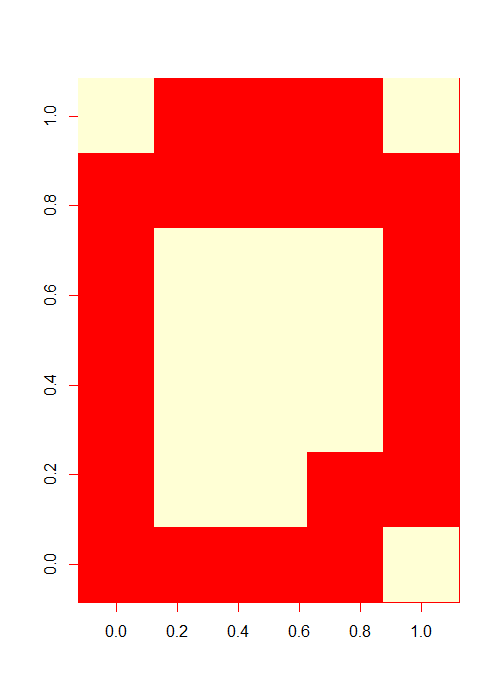
\includegraphics[width = \textwidth]{Figures/data0}
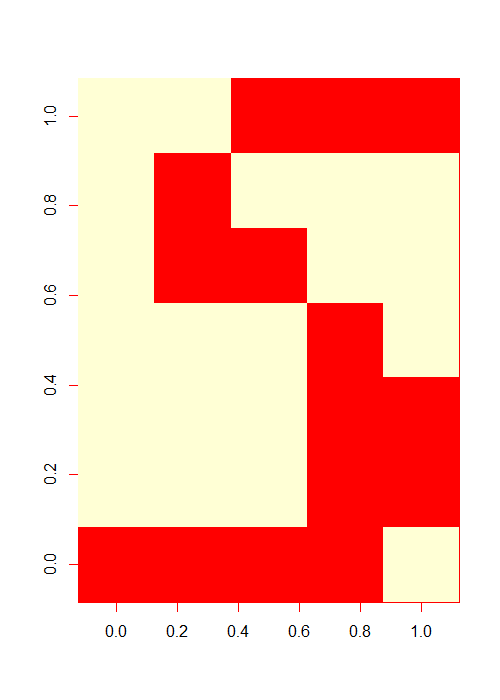
\includegraphics[width = \textwidth]{Figures/data5}
\end{minipage}
\begin{minipage}{0.2\linewidth}
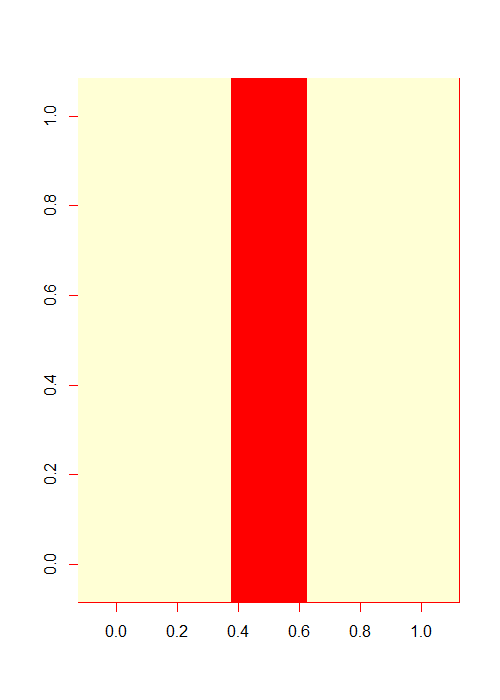
\includegraphics[width = \textwidth]{Figures/data1}
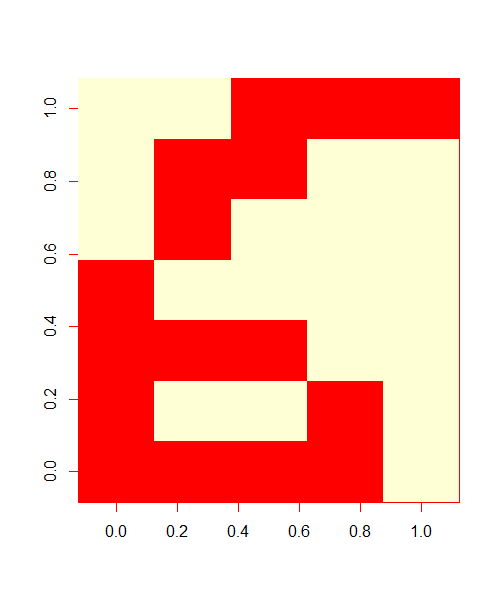
\includegraphics[width = \textwidth]{Figures/data6}
\end{minipage}
\begin{minipage}{0.2\linewidth}
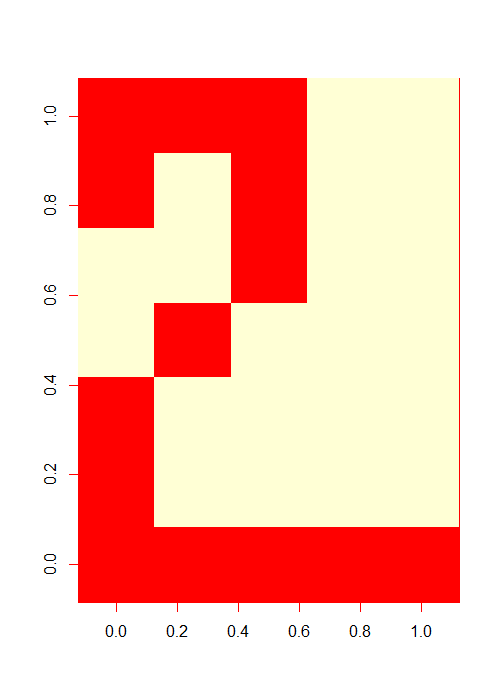
\includegraphics[width = \textwidth]{Figures/data2}
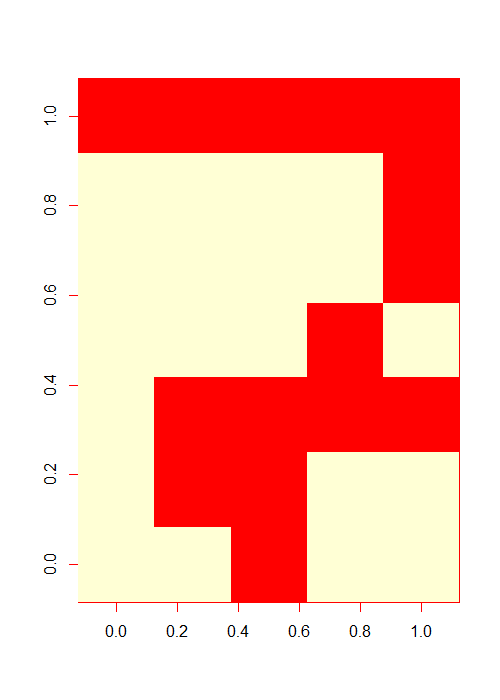
\includegraphics[width = \textwidth]{Figures/data7}
\end{minipage}
\begin{minipage}{0.2\linewidth}
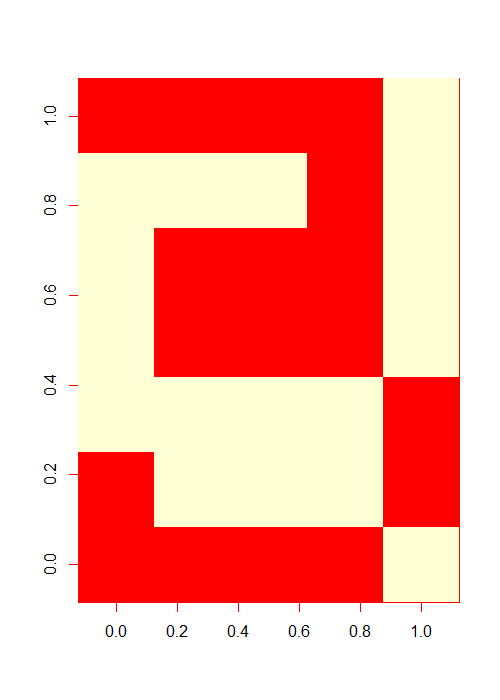
\includegraphics[width = \textwidth]{Figures/data3}
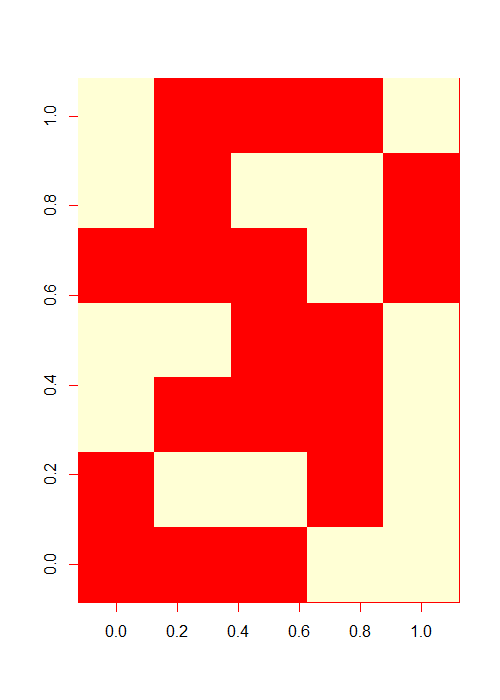
\includegraphics[width = \textwidth]{Figures/data8}
\end{minipage}
\begin{minipage}{0.2\linewidth}
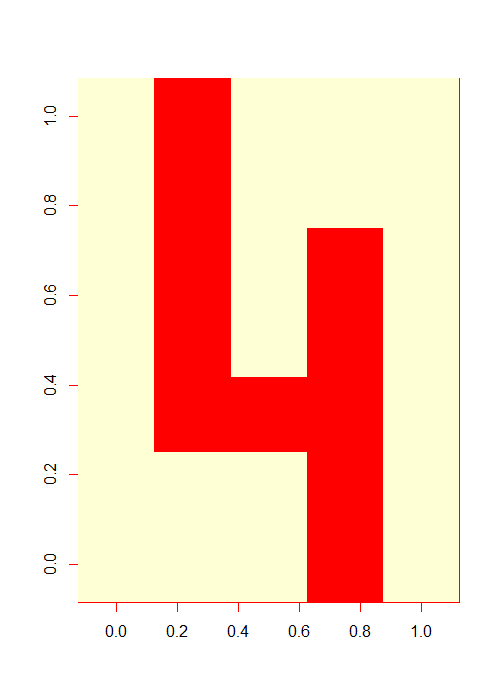
\includegraphics[width = \textwidth]{Figures/data4}
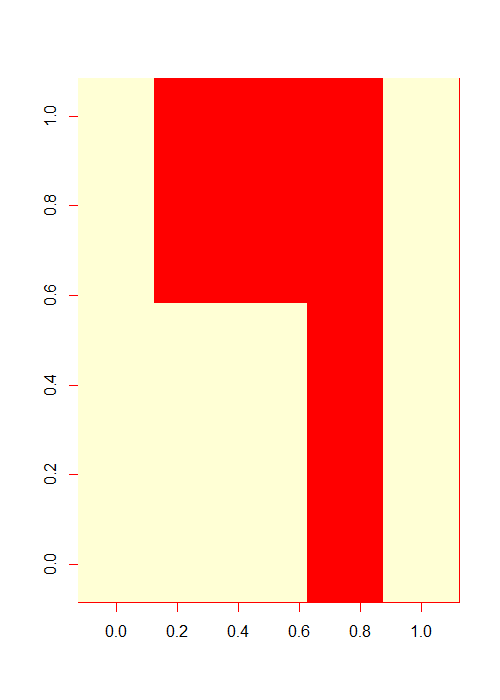
\includegraphics[width = \textwidth]{Figures/data9}
\end{minipage}




\paragraph{Les projections sur les axes} Une fois l'image reconstruite une projection sur l'axe $X$ et $Y$ sont effectuées, ce qui fournit deux vecteurs de caractéristiques supplémentaires.
\paragraph{Enveloppe de l'image} Sur chaque début et fin de ligne ou colonne des sondes récupèrent le premier pixel allumé à partir du bord où elles sont parties. Ce qui permet de reconstruire l'enveloppe du chiffre tracé. L'ensemble de ces informations sont concaténées dans un vecteur et fournies au réseau de neurones.


\subsubsection{Données vectorielles} Peu de temps a été alloué à la recherche de caractéristiques sur ce type de données c'est pourquoi seulement deux vecteurs de caractéristiques ont été extraits.

\paragraph{L'occurrence des orientations de tracé} À l'instar de l'image du tracé,  le nombre des différentes orientations prises lors du tracés est mémorisé et stocké dans un vecteur\footnote{Par exemple : trois fois vers le bas, une fois à gauche...}.
\paragraph{L'occurrence des variations} Il s'agit d'un vecteur qui contient le nombre de fois que le tracé a changé de direction et avec quel importance. Par exemple un « $1$ » aura souvent 0\degre de variation tandis qu'un « $6$ » aura souvent des variations du tracé entre 10\degre et 20\degre.


\paragraph{} Les caractéristiques extraites sont ensuite données au réseau de neurones pour l'entrainement.
\subsection{Méthodologie}
Afin de pouvoir obtenir le réseau de neurones le plus efficace possible, il était nécessaire d'estimer au mieux un certain nombre de méta-paramètres tels que le nombre de neurones dans la couche cachée, le nombre d'itérations lors de l'apprentissage et le pas $\eta$ pour l'estimation des poids.

\paragraph{Cross-validation} Pour toutes les étapes d'estimation des paramètres, les données d'entrainement étaient découpées en cinq. Quatre cinquièmes des données étaient alors utilisées pour l'entrainement d'un réseau de neurones, le dernier fragment de données étant utilisé pour la validation. Chaque fragment étant utilisé une fois pour la validation, cinq réseaux étaient entrainés.

À la fin de l'entrainement et de la validation de tous les réseaux, la MSE\footnote{Mean Square Error} et le taux de reconnaissance moyens étaient conservés.

\paragraph{Protocole} Pour chaque type de données, le protocole suivit était relativement le même :
\begin{enumerate}
\item Des réseaux de neurones sont entrainés en fixant le nombre d'itérations et de neurones, mais en faisant varier le pas $\eta$. Il est alors possible de trouver un optimum grâce aux MSE et aux taux de reconnaissance sur les données d'entrainement et de validation.
\item Le pas $\eta$ étant trouvé on peut le fixer et ré-entrainer des réseaux en faisant varier, cette fois, le nombre de neurones.
\item Même processus en faisant varier le nombre d'itération.
\item On ré-exécute le protocole du début avec les nouveaux paramètres afin de s'assurer qu'ils permettent de rester proche de l'optimal.
\end{enumerate} 

\paragraph{Problèmes rencontrés avec le protocole expérimental}
Un souci est rapidement apparu lors de l'entrainement des réseaux. En effet le protocole décrit ci-dessus semblait bien fonctionner lorsque les caractéristiques données en entrée du réseau de neurones étaient peu nombreuses et il était relativement aisé de repéré un optimum.

Mais l'augmentation du nombre de caractéristiques entraine une augmentation du poids des neurones cachés. Or, à partir d'un certain seuil, R refuse d'effectuer l'apprentissage des réseaux\footnote{Il serait apparemment possible d'augmenter ce seuil, mais il ne restait malheureusement pas assez de temps pour le vérifier et ré-entrainer les réseaux de neurones.}. De fait, les réseaux de neurones n'étaient jamais assez grand pour passer en sur-apprentissage (c.f. Figure \ref{fig:mse}), le MSE de validation ne divergeait jamais réellement ou, au mieux, stagnait.
\begin{figure}

\begin{minipage}{0.5\linewidth}
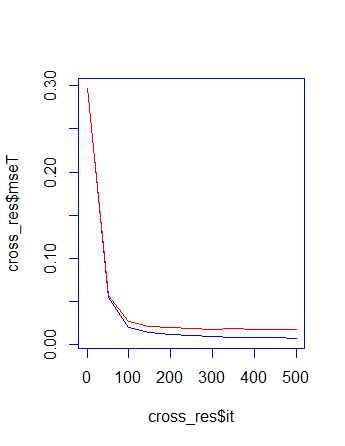
\includegraphics[width=\linewidth]{Figures/mse}
\label{fig:mse}
\end{minipage}
\begin{minipage}{0.5\linewidth}
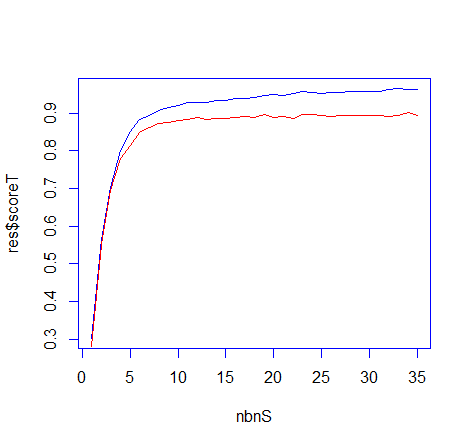
\includegraphics[width=\linewidth]{Figures/score_nn}
\label{fig:score}
\end{minipage}
\caption{MSE et taux de reconnaissance sur les données d'entrainement (bleu) et de validation (rouge).}
\end{figure}
\subsection{Résultats}

